    \subsection{Когомологии}

    Итак, рассмотрим цепной комплекс абелевых групп $(C_{\bullet}, \partial)$
    \[ \ldots \to C_{k} \to C_{k - 1} \to C_{k - 2} \to \ldots \]
    Тогда мы можем рассмотреть группы $C^{k} \eqdef \Hom\lr*{C_{k}, G}$, где $G$~--- фиксированная абелева группа.\footnote{В нашем, топологическом контексте, это группа коэффициентов.}
    Тогда мы получаем цепной комплекс
    \[ \ldots \leftarrow C^{k + 1} \xleftarrow{\delta} C^{k} \xleftarrow{\delta} C^{k - 1} \xleftarrow{\delta} \ldots \]
    Естественно, стрелки развернулись, так как мы подействовали на комплекс контравариантным функтором $\Hom(\_, G)$.
    Действие оператора $\delta$ определяется естественным образом:
    \[ \varphi \in C^{k}, \ \delta\varphi\colon C_{k + 1} \xrightarrow{\partial} C_{k} \xrightarrow{\varphi} G, \ \delta\varphi = \varphi \circ \partial. \]
    \begin{remark}
       Сразу же нетрудно заметить, что $\delta^2 = 0$, то есть построенный комплекс действительно будет комплексом. Действительно,
        \[ \delta_{k} \circ \delta_{k - 1}(\varphi(c)) = \delta_k(\varphi(\partial_{k - 1}c)) = \varphi(\partial_{k}\partial_{k - 1}c) = 0. \]
    \end{remark}

    \begin{definition}
        Группы гомологий коцепного комплекса $(C^{\bullet}, \delta) = (\Hom(C_{\bullet}), G), \delta)$ называют \emph{группами когомологий} комплекса $(C_{\bullet}, \partial)$ с коэффициентами в группе $G$ и обозначаются
    $H^{k}(C_{\bullet}; G)$. Как и в случае с гомологиями, $\Im{\delta_k}$ называют $k$-мерными кограницами, $\Ker{\delta_{k}}$~--- $k$-мерными коциклами, а  $C^k$~--- $k$-мерными коцепями.
    \end{definition}

    Таким образом, мы определили и \emph{сингулярные когомологии} пространства  $X$ (так как они строятся по сингулярным гомологиям).
    Заметим, что так как функтор $\Hom$ контравариантен, логично ожидать, что и когомологии будут контраваринатным функтором. Действительно,
    если $f\colon X \to Y$~--- непрерывное отображение, то у нас есть индуцированный морфизм
    \[ f_{*} \colon C_{k}(X) \to C_{k}(Y) \]
    и действием функтора $\Hom$ мы получаем индуцированный морфизм $f^{*}\colon C^{k}(Y) \to C^{k}(X)$:
    \[  \varphi \in C^{k}(Y), \ \varphi \colon C^{k}(Y) \to G, \ f^{*}(\varphi) \eqdef \varphi \circ f \colon C^{k}(X) \to G, \ f^{*}(\varphi) \in C^{k}(X). \]
    Покажем теперь, что у нас будет и индуцированный морфизм в когомологиях:
    \[ f^{*}\colon H^{k}(Y) \to H^{k}(X) \]
    Для этого надо проверить, что  отображение уважает добавление кограницы, то есть, если мы выберем
    другого представителя того же когомологического класса, мы полужем тот же образ, что и до этого. Действительно,
    \[ f^{*}(c_k + \delta c_{k - 1}) = f^{*}(c_k) + \delta f^{*}(c_{k - 1}) \]

    \begin{remark}
       Формально, как и в гомологиях, нам надо проверить, что $f^{*}\delta = \delta f^{*}$. Действительно, пусть $\varphi \in C^{k}(X)$, тогда
        \[ f^{*}(\delta \varphi) = f^{*}(\varphi  \partial)  = \varphi \partial f = \varphi f \partial = \delta f^{*}(\varphi). \]
        В третьем равенстве мы пользуемся тем, что в начале курса мы уже проверяли, что граничный оператор коммутирует с непрерывными отображениями.
    \end{remark}

    \subsection{Формула универсальных коэффициентов для когомологий}

    \begin{example}\label{TorsionCohomology}
        Рассмотрим следующий комплекс:
        \[ 0 \to \underbrace{\Z}_{C_{3}} \xrightarrow{\cdot 0} \underbrace{\Z}_{C_2} \xrightarrow{\cdot 2} \underbrace{\Z}_{C_1} \xrightarrow{\cdot 0} \underbrace{\Z}_{C_0} \to 0 \]
        После применения функтора $\Hom(\_, \Z)$ мы получим такой комплекс:
        \[ 0 \leftarrow \underbrace{\Z}_{C^3} \xleftarrow{} \underbrace{\Z}_{C^2} \xleftarrow{} \underbrace{\Z}_{C^1} \xleftarrow{} \underbrace{\Z}_{C^0} \leftarrow 0\]
        Посмотрим, какие в новом комплексе отображения. Действительно, пусть $\varphi\colon C_{1} \to \Z $, $\psi\colon C_2 \to C_1, \psi(x) = 2x$, тогда
        $\varphi \psi\colon C_2 \to \Z \in C^{2}$. Нетрудно заметить, что $\varphi(\psi(x)) = \varphi(2x) = 2\varphi(x)$.
        Значит, мы получили вот такой комплекс:
        \[ 0 \leftarrow \underbrace{\Z}_{C^3} \xleftarrow{\cdot 0} \underbrace{\Z}_{C^2} \xleftarrow{\cdot 2} \underbrace{\Z}_{C^1} \xleftarrow{\cdot 0} \underbrace{\Z}_{C^0} \leftarrow 0\]
        Вычислим сначала гомологии:
        \[ H_{0}(C_{\bullet}) = \Z, \ H_{1}(C_{\bullet}) = \Z/2\Z, \ H_{2}(C_{\bullet}) = 0, \ H_{3}(C_{\bullet}) = \Z. \]
        Теперь вычислим когомологии:
        \[ H^{0}(C_{\bullet}) = \Z, \ H^{1}(C_{\bullet}) = 0,\  H_{2}(C_{\bullet}) = \Z/2\Z,\  H_{3}(C_{\bullet}) = \Z. \]

        То есть, сами группы не изменились, но изменилась градуировка.

        Это вполне естественно, так как, на самом деле, любой цепной комплекс конечно-порожденных свободных абелевых групп является прямой суммой
        комплексов
        \[ 0 \to \Z \to 0 \text{ и } 0 \to \Z \xrightarrow{\cdot m} \Z \to 0 \]
        и в силу того, что функтор $\Hom$ аддитивен на конечных копроизведениях, применяя $\Hom(\_, \Z)$ к исходному комплексу, мы получаем прямую  сумму комплексов
        \[ 0 \leftarrow \Z \leftarrow 0 \text{ и } 0 \leftarrow \Z \xleftarrow{\cdot m} \Z \leftarrow 0 \]

        Таким образом, мораль всего этого дела в том, что группы когомологий~--- тоже самое, что группы гомологий, за исключением того, что кручение смещается на олну размерность.
    \end{example}

    \begin{statement}
        Пусть $(C_{\bullet}, \partial)$~--- цепной комплекс. Тогда существует гомоморфизм
        \[ h\colon H^{n}(C; G) \to \Hom\lr*{H_n(C), G}. \]
    \end{statement}
    \begin{proof}
        Рассмотрим когомологический класс  $[\varphi] \in H^{n}(C_{\bullet}; G)$, $\varphi\colon C_n \to G$, $\delta \varphi = 0$.
        \[ \delta \varphi = \varphi \partial \Leftrightarrow \varphi\vert_{\Im{\partial_{n + 1}}} = 0\]
        Ограничение $\varphi_0 = \varphi\vert_{\Ker{\partial_{n}}} \colon \Ker{\partial_n} \to G$ индуцирует гомоморфизм факторизации
        \[ \overline{\varphi_0} \colon \Ker{\partial_n}/\Im{\partial_{n + 1}} \to G, \quad \overline{\varphi_0} \in \Hom\lr{H_{n}(C_{\bullet}), G}.\]
        Таким образом, полагая $h(\varphi) = \overline{\varphi}_0$, мы получаем нужное.
    \end{proof}

    \bf{Упражнение.} $h$~--- эпиморфизм.

    Рассмотрим теперь короткую точную последовательность
    \[ 0 \to Z_{n + 1} \to C_{n + 1} \xrightarrow{\partial} B_{n} \to 0\]
    Применяя функтор $\Hom(-, G)$ мы получаем точную последовательность
    \[ 0 \leftarrow Z^{n + 1} \leftarrow C^{n + 1} \leftarrow B^{n + 1} \leftarrow 0 \]
    На самом деле, мы имеем коммутативную диаграмму
    \begin{center}
        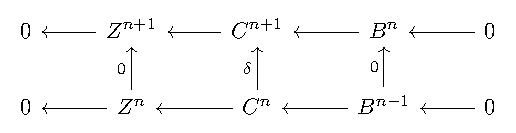
\includegraphics{lectures/0/pictures/cd_13}
    \end{center}

    Видно, что эта диаграмма~--- часть короткой точной последовательности комплексов. Она даёт нам длинную точную последовательность:
    \[ \ldots \leftarrow B^{n} \leftarrow Z^{n} \leftarrow H^n\lr*{C_{\bullet}, G} \leftarrow B^{n - 1} \leftarrow Z^{n - 1} \leftarrow \ldots \]
    Разбивая длинную точную последовательность на короткие точные последовательности мы получаем:
    \[ 0 \leftarrow \Ker\lr*{Z^n \to B^n} \xleftarrow{h} H^n\lr*{C_{\bullet}; G} \leftarrow \Coker\lr*{Z^{n - 1} \to B^{n - 1}} \leftarrow 0\]
    А теперь заметим, что  $\Ker\lr*{Z^n \to B^n} = \Hom\lr*{H_{n}(C_{\bullet}), G}$. Таким образом, мы получаем  расщепимую точную последовательность:
    \[ 0 \to \Coker\lr*{Z^{n - 1} \to B^{n - 1}}  \to H^n\lr*{C_{\bullet}; G} \to \Hom\lr*{H_{n}(C_{\bullet}), G} \to 0. \]
    
    \begin{definition}
        Пусть $H$~--- абелева группа. Тогда её \emph{свободная резольвента}~--- это точная последовательность
        \[ \ldots \to F_{2} \xrightarrow{f_2} F_{1} \xrightarrow{f_1} F_0 \xrightarrow{f_0} H \to 0, \]
        в которой каждая группа $F_n$ свободная.
    \end{definition}

    Применяя к этой точной последовательности функтор $\Hom(-, G)$  мы можем потерять точность, но во всяком случае, получим цепной комплекс:
    \[ \leftarrow F_2^* \xleftarrow{f_2^*} F_1^* \xleftarrow{f_1^*} F_0^* \xleftarrow{f_0^*} H^* \leftarrow 0\]

    Будем обозначать группы когомологий свободной резольвенты, как $H^n(F, G)$. Нам понадобится следующее утверждение из гомологической алгебры:

    \begin{lemma}\label{FreeResolventProp}
        Пусть даны свободные резольвенты $F$ и $F'$ абелевых групп $H$ и $H'$. Тогда любой гомоморфизм $\alpha\colon H \to H'$
        можно продолжить до цепного отображения $F \to F'$. Кроме того, любые два таких цепных отображения, продолжающие гомоморфизм $\alpha$, цепно гомотопны.

        Для любых двух свободных резольвент $F$ и $F'$ группы $H$ существуют канонические изоморфизмы
        \[ H^n(F; G) \cong H^n(F'; G). \]
    \end{lemma}

    У любой абелевой группы $H$ есть свободная резольвента вида
    \[ 0 \to F_1 \to F_0 \to H \to 0 \]
    с $F_i = 0$ при $i > 1$, которую мы сейчас построим.

    Выберем в $H$ набор образующих и пусть $F_0$~--- группа, свободно порожденная этими образующими.
    Тогда у нас есть сюръективный гомоморфизм $f_0\colon F_0 \to H$, переводящий элементы базиса в образующие $H$. Его ядро будет свободно, как
    подгруппа свободной группы, поэтому мы можем положить $F_1 = \Ker{f_0}$, а в качестве $f_1$ взять включение $\Ker{f_0} \hookrightarrow F_0$.

    Для этой свободной резольвенты мы имеем $H^n(F; G) = 0 \ \forall n > 1$, поэтому, из леммы~\ref{FreeResolventProp}  мы получаем, что это
    должно быть верно для всех свободных резольвент.

    Таким образом, единственная интересная группа из $H^n(F; G)$~--- это $H^1(F; G)$. Эта группа зависит лишь от $H$ и $G$, поэтому
    обычно её обозначают $\Ext(H, G)$\footnote{Вообще говоря, в гомологической алгебре функтор $\Ext$ обычно интерпретируют, как множество классов эквивалентности расширений $G$ посредством $H$, но в алгебраической топологии такая интерпретация редко нужна. }.

    Так вот, из построения свободной резольвенты для группы $H$ и определения когомологий мы теперь наконец можем заметить, что
    \[ \Coker\lr*{Z^{n - 1} \to B^{n - 1}} = \Ext\lr*{H_{n - 1}(C_{\bullet}), G}. \]

    Теперь мы наконец можем заключить, что мы доказали формулу универсальных коэффициентов для когомологий:

    \begin{theorem}[Об универсальных коээфициентах для когомологий]
        Пусть $C_{\bullet}$~--- цепной комплекс. Тогда его группы когомологий определяются расщепимыми короткими точными последовательностями
        \[ 0 \to \Ext\lr*{H_{n - 1}(C_{\bullet}), G} \to H^{n}(C; G) \to \Hom\lr*{H_{n}(C), G} \to 0 \]
    \end{theorem}

    Вообще говоря, это утверждение достаточно полезно, потому что на конечнопорожденных абелевых группах функтор $\Ext$ несложно посчитать:
    \begin{itemize}
        \item $\Ext\lr*{H \oplus H', G} \cong \Ext\lr*{H, G} \oplus \Ext\lr*{H', G}$.
        \item $\Ext\lr*{H, G} = 0$, если $H$~--- свободна.
        \item $\Ext(\Z/n\Z, G) \cong G/nG$.
        \item Если $H$ конечно порождена, то имеет место изоморфизм
         \[ \Ext(H, \Z) \cong \mathrm{Tor}\lr*{H}. \]
    \end{itemize}

    Кроме того, теорема об универсальных коэффициентов позволяет вычислять когомологии, зная только гомологии.
    \begin{corollary}
        Если группы гомологий $H_n(C)$ и $H_{n - 1}(C)$ комплекса $C$, состоящего из свободных абелевых групп, конечно порождены и $T_n \subset H_n$ и $T_{n - 1} \subset H_{n - 1}$~--- подгруппы кручения, то
        \[ H^{n}\lr*{C; \Z} \cong (H_{n - 1}(C)/T_n) \oplus T_{n - 1}.\]
    \end{corollary}

    Это следствие даёт нам обобщение и формализацию примера~\ref{TorsionCohomology}.

    Кроме того, из всего этого дела есть еще одно замечательное следствие:

    \begin{corollary}
        Если $f\colong C_{\bullet} \to C_{\bullet}'$ индуцирует изоморфизм всех групп гомологий $H_{k}(C_{\bullet}) \cong H_{k}\lr*{C_{\bullet}'}$.
        Тогда отображения $f^{*}\colon H^{k}\lr*{C_{\bullet}; G} \cong H^{k}\lr*{C_{\bullet}'; G}$.
    \end{corollary}
    \begin{proof}
        Действительно, достаточно заметить, что из свойств свободной резольвенты мы знаем, что отобрежение цепных комплексов индуцирует такую вот диаграмму:
        \begin{center}
            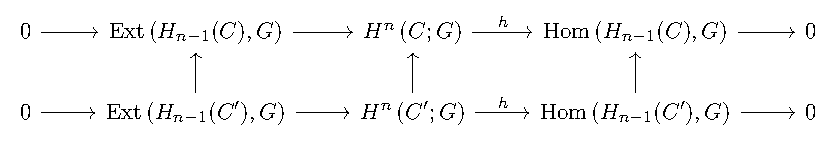
\includegraphics{lectures/0/pictures/cd_14}
        \end{center}
        Применяя 5-лемму и индукцию, мы получаем нужное.
    \end{proof}

    \subsection{Умножение в когомологиях}

